\documentclass[a4paper,11pt]{jsarticle}

% 英文化
\usepackage[english]{babel}
% 数式
\usepackage{amsmath,amsfonts}
\usepackage{amsthm}
\usepackage{bm}
% 画像
\usepackage[dvipdfmx]{graphicx}
% 箇条書き
\usepackage{enumitem}
% 枠付き文章
\usepackage{ascmac}

\SetLabelAlign{Center}{\hfil#1\hfil}
\SetLabelAlign{CenterWithParen}{\hfil(\makebox[1.0em]{#1})\hfil}

\begin{document}

\title{%
  Fenchel Duality  \\
  \large 3.1 Subgradients and Convex Functions}
\author{Ryota Iwamoto}
\date{\today}
\maketitle

We use the book; Convex Analysis and Nonlinear Optimization (author: J.M.BORWEIN and A.S.LEWIS), pp.33-36.

\begin{quote}
  Quote:

  We have already seen, in the First order sufficient condition (2.1.2), one
  benefit of convexity in optimization: critical points of convex functions are
  global minimizers. In this section we extend the types of functions we
  consider in two important ways:

  \qquad
    \begin{enumerate}[label=\roman*,align=CenterWithParen]
      \item We do not require $f$ to be differentiable.
      \item We allow $f$ to take the value $+\infty$.
    \end{enumerate}
\end{quote}

This book Chapter 2 explains a optimization of convex functions with good conditions, which is differentiable and not including infinity points. In this section, we consider extended functions like being not differentiable and allowed to take the value $+\infty$.

\begin{quote}
  Quote:

  Our derivation of first order conditions in Section 2.3  illustrates the utility of considering nonsmooth functions even in the context of smooth problems. Allowing the value $+\infty$ lets us rephrase a problem like
$$ \inf \text{$\{ g(x)\:|\:x \in{C}\}$} $$
as $ \inf \text{$(g+\delta_C)$} $, where the indicator function $\delta_C$($x$) is 0 for $x$ in $C$ and $+\infty$
otherwise.

\end{quote}

Here We consider the definition of indicator function.

% タイトルの位置は,カギ括弧[]の中で指定します.l:左,c:中央,r:右にタイトルが書かれます.
\begin{itembox}[l]{\underline{Definition (Indicator Funciton) }}
  The indicator function of a set $C$ of $\mathbb{E}$, denoted by $\delta_C$, is defined by

  \begin{equation}
    \delta_C(x)=
    \begin{cases}
      0 & if\:x \in{C}, \\
      \infty & if\:otherwise. \notag
    \end{cases}
  \end{equation}
\end{itembox}

\begin{quote}
  Quote:

  The domain of a function $f$ : $\mathbb{E}$ → $ \left ( -\infty ,+\infty \right ] $ is the set

  \begin{equation}
    dom f = \{x \in{\mathbb{E}}\:|\:f(x) < +\infty \}. \notag
  \end{equation}
  We say $f$ is convex if it is convex on its domain, and proper if its domain
  is nonempty. We call a function $g$ : $\mathbb{E}$ → $ \left [ -\infty ,+\infty \right ) $ concave if $-g$ is
  convex, although for reasons of simplicity we will consider primarily convex
  functions. If a convex function $f$ satisfies the stronger condition

  \begin{equation}
    f(\lambda x + \mu y) \leq \lambda f(x) + \mu f(y),\:for \:all\: x, y \in{\mathbb{E}},\: \lambda, \mu \in{\mathbb{R}}_+ \notag
  \end{equation}

  we say $f$ is $sublinear$. If $f(\lambda x) = \lambda f(x)$ for all $x$ in $\mathbb{E}$ and $\lambda$ in ${\mathbb{R}}_+$ then
  $f$ is $positively\:homogeneous$: in particular this implies $f(0) = 0$. (Recall the convention 0 · (+$\infty$) = 0.) If $ f(x + y) \leq f(x) +  f(y) $ for all $x$ and $y
$  in $\mathbb{E}$ then we say $f$ is $subadditive$. It is immediate that if the function $f$
  is sublinear then $-f(x) \leq f(-x)$ for all $x$ in $\mathbb{E}$. The $lineality\:space$ of a
  sublinear function $f$ is the set

  \begin{equation}
    lin f = \{x \in \mathbb{E}\:|\:-f(x) = f(-x)\}. \notag
  \end{equation}

\end{quote}

We describe some definitions and the figure below.

\begin{itembox}[l]{\underline{Definition (Sublinear) }}
  A convex function $f$ is \textbf{sublinear} if this $f$ satisfies the condition

  \begin{equation}
    f(\lambda x + \mu y) \leq \lambda f(x) + \mu f(y),\:for \:all\: x, y \in{\mathbb{E}},\: \lambda, \mu \in{\mathbb{R}}_+. \notag
  \end{equation}
\end{itembox}

Figure:

\begin{equation}
  f(x, y)=
  \begin{cases}
    2|x| + y & if\:y \leq 0, \\
    2|x| + 6y & if\:y > 0. \notag
  \end{cases}
\end{equation}

\begin{center}
  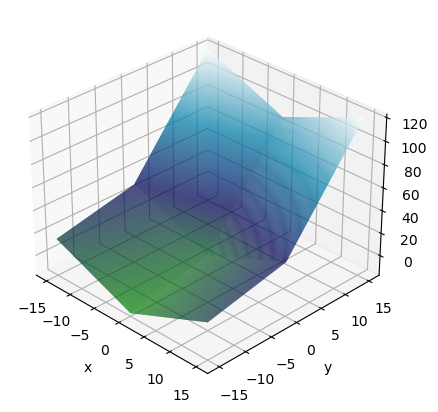
\includegraphics[width=8cm]{sublinear_output.png}
\end{center}

\begin{itembox}[l]{\underline{Definition (Positively Homogeneous and Subadditive) }}
  A convex function $f$ is \textbf{positively homogeneous} if this $f$ satisfies the condition

  \begin{equation}
    f(\lambda x) = \lambda f(x),\:for \:all\: x \in{\mathbb{E}},\: \lambda \in{\mathbb{R}}_+. \notag
  \end{equation}

  And a convex function $f$ is \textbf{subadditive} if this $f$ satisfies the condition

  \begin{equation}
    f( x + y) \leq f(x) + f(y),\:for \:all\: x, y \in{\mathbb{E}}. \notag
  \end{equation}
\end{itembox}

\begin{itembox}[l]{\underline{Proposition }}
  If the function $f$
  is sublinear then $-f(x) \leq f(-x)$ for all $x$ in $\mathbb{E}$.
\end{itembox}

\begin{proof}
  We show that it holds $-f(x) \leq f(-x)$ for all $x$ in $\mathbb{E}$.

  By the assumption of sublinear of $f$, we can use the inequality

  \begin{equation}
    f(\lambda x + \mu y) \leq \lambda f(x) + \mu f(y),\:for \:all\: x, y \in{\mathbb{E}},\: \lambda, \mu \in{\mathbb{R}}_+. \notag
  \end{equation}

  For any $x$ and $y$, we take $y=-x$ since ${\mathbb{E}}$ is a vector space, and also take $\lambda=\mu=1$. These values and the above assumption, we get the inequality

  \begin{equation}
    f(x + (-x)) \leq f(x) + f(-x). \notag
  \end{equation}

  By $f(0) = 0$,

  \begin{equation}
    0 \leq f(x) + f(-x). \notag
  \end{equation}

  Therefore we got $-f(x) \leq f(-x)$ for all $x$ in $\mathbb{E}$.
\end{proof}

\begin{itembox}[l]{\underline{Definition (Lineality Space) }}
  The $lineality\:space$ of a
  sublinear function $f$, denoted by $lin f$, is the set

  \begin{equation}
    lin f = \{x \in \mathbb{E}\:|\:-f(x) = f(-x)\}. \notag
  \end{equation}
\end{itembox}

\end{document}
